% ============================================================
% 讲义 — 人教版高二选择性必修第一册 第1章 空间向量与立体几何
% 编译命令：xelatex -interaction=nonstopmode 文件名.tex
% ============================================================
\documentclass[12pt, a4paper]{ctexart}
\usepackage[margin=2.2cm]{geometry}
\usepackage{amsmath, amssymb}
\usepackage{enumitem}
\usepackage{tcolorbox}
\usepackage{booktabs}
\usepackage{array}
\usepackage{fancyhdr}
\usepackage{xcolor}
\usepackage{tikz}
\usepackage{hyperref}
\usepackage{graphicx}
\usepackage{multirow}
\usepackage{pgfplots}
\pgfplotsset{compat=1.18}
\usetikzlibrary{3d, calc, arrows.meta, positioning}

% 颜色定义
\definecolor{mainblue}{RGB}{41, 98, 168}
\definecolor{lightblue}{RGB}{230, 240, 255}
\definecolor{tipgreen}{RGB}{34, 139, 87}
\definecolor{lightgreen}{RGB}{235, 250, 240}
\definecolor{warnred}{RGB}{200, 50, 50}
\definecolor{lightred}{RGB}{255, 240, 240}
\definecolor{examorange}{RGB}{210, 120, 20}
\definecolor{lightorange}{RGB}{255, 248, 235}
\definecolor{apppurple}{RGB}{120, 60, 170}
\definecolor{lightpurple}{RGB}{245, 238, 255}

% 页眉页脚
\pagestyle{fancy}
\fancyhf{}
\fancyhead[L]{\small\textcolor{mainblue}{\textbf{人教版高二选必1 · 第1章 空间向量与立体几何}}}
\fancyhead[R]{\small\textcolor{mainblue}{空间向量与立体几何讲义}}
\fancyfoot[C]{\small —\ \thepage\ —}
\renewcommand{\headrulewidth}{0.6pt}
\renewcommand{\headrule}{\hbox to\headwidth{\color{mainblue}\leaders\hrule height \headrulewidth\hfill}}
\renewcommand{\footrulewidth}{0pt}

% tcolorbox 样式
\newtcolorbox{knowledgebox}[1][]{%
  colback=lightblue, colframe=mainblue,
  fonttitle=\bfseries\large, title=#1,
  arc=3mm, boxrule=0.8pt,
  left=8pt, right=8pt, top=6pt, bottom=6pt
}

\newtcolorbox{tipbox}[1][]{%
  colback=lightgreen, colframe=tipgreen,
  fonttitle=\bfseries, title=#1,
  arc=2mm, boxrule=0.6pt,
  left=6pt, right=6pt, top=4pt, bottom=4pt
}

\newtcolorbox{warnbox}[1][]{%
  colback=lightred, colframe=warnred,
  fonttitle=\bfseries, title=#1,
  arc=2mm, boxrule=0.6pt,
  left=6pt, right=6pt, top=4pt, bottom=4pt
}

\newtcolorbox{examplebox}[1][]{%
  colback=lightorange, colframe=examorange,
  fonttitle=\bfseries, title=#1,
  arc=3mm, boxrule=0.8pt,
  left=8pt, right=8pt, top=6pt, bottom=6pt
}

\newtcolorbox{appbox}[1][]{%
  colback=lightpurple, colframe=apppurple,
  fonttitle=\bfseries, title=#1,
  arc=3mm, boxrule=0.8pt,
  left=8pt, right=8pt, top=6pt, bottom=6pt
}

\setCJKmainfont{Hiragino Sans GB}
\setCJKsansfont{Heiti SC}

\begin{document}

% ============ 标题页 ============
\begin{center}
{\Huge\bfseries\textcolor{mainblue}{第1章\quad 空间向量与立体几何}}\\[12pt]
{\Large\textcolor{gray}{讲\quad 义}}\\[8pt]
\rule{0.6\textwidth}{1pt}\\[8pt]
{\normalsize 适用：人教版\quad 高二选择性必修第一册\quad |\quad 课时：4课时}
\end{center}
\vspace{10pt}

% ================================================================
%  第一部分：知识点讲解
% ================================================================
\section*{\textcolor{mainblue}{一、知识点讲解}}

% -------------------- 1.1 空间向量及其运算 --------------------
\subsection*{1.1\quad 空间向量及其运算}

\begin{knowledgebox}[空间向量的概念]
在空间中，既有\textbf{大小}又有\textbf{方向}的量叫做\textbf{空间向量}，记作$\vec{a}$或$\overrightarrow{AB}$。
空间向量的大小叫做向量的\textbf{模}（长度），记作$|\vec{a}|$或$|\overrightarrow{AB}|$。

模为$0$的向量叫做\textbf{零向量}，记作$\vec{0}$。模为$1$的向量叫做\textbf{单位向量}。

方向相同且模相等的两个向量叫做\textbf{相等向量}。方向相反且模相等的两个向量互为\textbf{相反向量}。
\end{knowledgebox}

\begin{knowledgebox}[空间向量的线性运算]
\textbf{加法（三角形法则 / 平行四边形法则）}：
\[
\overrightarrow{AB}+\overrightarrow{BC}=\overrightarrow{AC}
\]
满足交换律 $\vec{a}+\vec{b}=\vec{b}+\vec{a}$ 和结合律 $(\vec{a}+\vec{b})+\vec{c}=\vec{a}+(\vec{b}+\vec{c})$。

\textbf{减法}：$\vec{a}-\vec{b}=\vec{a}+(-\vec{b})$。

\textbf{数乘}：$\lambda\vec{a}$（$\lambda\in\mathbb{R}$）
\begin{itemize}[nosep]
  \item $\lambda>0$ 时方向与 $\vec{a}$ 相同，$|\lambda\vec{a}|=\lambda|\vec{a}|$
  \item $\lambda<0$ 时方向与 $\vec{a}$ 相反，$|\lambda\vec{a}|=|\lambda|\cdot|\vec{a}|$
  \item $\lambda=0$ 时 $\lambda\vec{a}=\vec{0}$
\end{itemize}
满足结合律 $\lambda(\mu\vec{a})=(\lambda\mu)\vec{a}$ 和分配律 $\lambda(\vec{a}+\vec{b})=\lambda\vec{a}+\lambda\vec{b}$。
\end{knowledgebox}

\begin{knowledgebox}[空间向量的数量积]
\textbf{定义}：设 $\vec{a}$、$\vec{b}$ 是两个空间向量，它们的夹角为 $\theta$（$0\le\theta\le\pi$），则
\[
\vec{a}\cdot\vec{b}=|\vec{a}|\,|\vec{b}|\cos\theta
\]
\textbf{性质}：
\begin{itemize}[nosep]
  \item $\vec{a}\cdot\vec{a}=|\vec{a}|^2$
  \item $\vec{a}\perp\vec{b}\iff\vec{a}\cdot\vec{b}=0$
  \item $\cos\theta=\dfrac{\vec{a}\cdot\vec{b}}{|\vec{a}|\,|\vec{b}|}$
\end{itemize}
\textbf{运算律}：$\vec{a}\cdot\vec{b}=\vec{b}\cdot\vec{a}$；$(\lambda\vec{a})\cdot\vec{b}=\lambda(\vec{a}\cdot\vec{b})$；$\vec{a}\cdot(\vec{b}+\vec{c})=\vec{a}\cdot\vec{b}+\vec{a}\cdot\vec{c}$。

\textbf{注意}：数量积不满足结合律，即 $(\vec{a}\cdot\vec{b})\cdot\vec{c}\ne\vec{a}\cdot(\vec{b}\cdot\vec{c})$ 一般不成立。
\end{knowledgebox}

\begin{warnbox}[易错提醒]
\begin{enumerate}[nosep]
  \item 数量积 $\vec{a}\cdot\vec{b}$ 的结果是一个\textbf{标量}（实数），不是向量。
  \item $\vec{a}\cdot\vec{b}=0$ 不能直接推出 $\vec{a}=\vec{0}$ 或 $\vec{b}=\vec{0}$，也可能是 $\vec{a}\perp\vec{b}$。
  \item 向量的夹角 $\theta$ 取值范围是 $[0,\pi]$，不是 $[0,2\pi)$。
\end{enumerate}
\end{warnbox}

% -------------------- 1.2 空间向量基本定理 --------------------
\subsection*{1.2\quad 空间向量基本定理}

\begin{knowledgebox}[共面向量定理]
如果两个向量 $\vec{a}$、$\vec{b}$ 不共线，则向量 $\vec{p}$ 与 $\vec{a}$、$\vec{b}$ 共面的充要条件是：存在唯一的实数对 $(x,y)$，使得
\[
\vec{p}=x\vec{a}+y\vec{b}
\]
\end{knowledgebox}

\begin{knowledgebox}[空间向量基本定理]
设 $\vec{e}_1$、$\vec{e}_2$、$\vec{e}_3$ 是空间中三个\textbf{不共面}的向量，则对空间中任意向量 $\vec{p}$，存在唯一的有序实数组 $(x,y,z)$，使得
\[
\vec{p}=x\vec{e}_1+y\vec{e}_2+z\vec{e}_3
\]
其中 $\{\vec{e}_1,\vec{e}_2,\vec{e}_3\}$ 叫做空间的一个\textbf{基底}。

当 $\vec{e}_1$、$\vec{e}_2$、$\vec{e}_3$ 为两两垂直的单位向量时，称为\textbf{标准正交基}（单位正交基底），记作 $\{\vec{i},\vec{j},\vec{k}\}$。
\end{knowledgebox}

\begin{tipbox}[规律总结]
在空间中选取基底时，优先选择\textbf{共起点、不共面}的三个向量。在长方体或正方体中，通常选取从同一顶点出发的三条棱所在向量作为基底。
\end{tipbox}

% -------------------- 1.3 空间向量的坐标运算 --------------------
\subsection*{1.3\quad 空间向量的坐标运算}

\begin{knowledgebox}[空间直角坐标系]
在空间中选定一点 $O$ 和一个单位正交基底 $\{\vec{i},\vec{j},\vec{k}\}$，以 $O$ 为原点，分别以 $\vec{i}$、$\vec{j}$、$\vec{k}$ 的方向为 $x$ 轴、$y$ 轴、$z$ 轴的正方向，建立\textbf{空间直角坐标系} $Oxyz$。

空间中点 $P$ 的坐标记为 $(x,y,z)$。设 $A(x_1,y_1,z_1)$、$B(x_2,y_2,z_2)$，则
\[
\overrightarrow{AB}=(x_2-x_1,\;y_2-y_1,\;z_2-z_1)
\]
\end{knowledgebox}

\begin{knowledgebox}[坐标运算法则]
设 $\vec{a}=(a_1,a_2,a_3)$，$\vec{b}=(b_1,b_2,b_3)$，$\lambda\in\mathbb{R}$，则

\begin{center}
\renewcommand{\arraystretch}{1.4}
\begin{tabular}{ll}
\toprule
运算 & 公式 \\
\midrule
加法 & $\vec{a}+\vec{b}=(a_1+b_1,\;a_2+b_2,\;a_3+b_3)$ \\
减法 & $\vec{a}-\vec{b}=(a_1-b_1,\;a_2-b_2,\;a_3-b_3)$ \\
数乘 & $\lambda\vec{a}=(\lambda a_1,\;\lambda a_2,\;\lambda a_3)$ \\
数量积 & $\vec{a}\cdot\vec{b}=a_1b_1+a_2b_2+a_3b_3$ \\
模 & $|\vec{a}|=\sqrt{a_1^2+a_2^2+a_3^2}$ \\
夹角 & $\cos\theta=\dfrac{a_1b_1+a_2b_2+a_3b_3}{\sqrt{a_1^2+a_2^2+a_3^2}\;\sqrt{b_1^2+b_2^2+b_3^2}}$ \\
\bottomrule
\end{tabular}
\end{center}

\textbf{平行条件}：$\vec{a}\parallel\vec{b}\iff\dfrac{a_1}{b_1}=\dfrac{a_2}{b_2}=\dfrac{a_3}{b_3}$（分母不为零时）。

\textbf{垂直条件}：$\vec{a}\perp\vec{b}\iff a_1b_1+a_2b_2+a_3b_3=0$。
\end{knowledgebox}

\begin{knowledgebox}[空间两点间距离公式]
设 $A(x_1,y_1,z_1)$、$B(x_2,y_2,z_2)$，则
\[
|AB|=\sqrt{(x_2-x_1)^2+(y_2-y_1)^2+(z_2-z_1)^2}
\]
\end{knowledgebox}

% -------------------- 1.4 用向量方法研究直线与平面的位置关系 --------------------
\subsection*{1.4\quad 用向量方法研究直线与平面的位置关系}

\begin{knowledgebox}[直线的方向向量与平面的法向量]
\textbf{直线的方向向量}：直线 $l$ 上的非零向量 $\vec{v}$ 称为 $l$ 的方向向量。一条直线的方向向量不唯一，它们互相平行。

\textbf{平面的法向量}：垂直于平面 $\alpha$ 的非零向量 $\vec{n}$ 称为 $\alpha$ 的法向量。一个平面的法向量不唯一，它们互相平行。

\medskip
\textbf{求平面法向量的方法}：设平面 $\alpha$ 内两个不共线的向量为 $\vec{a}$ 和 $\vec{b}$，平面的法向量为 $\vec{n}=(x,y,z)$，则由
\[
\begin{cases}\vec{n}\cdot\vec{a}=0\\\vec{n}\cdot\vec{b}=0\end{cases}
\]
可解出法向量 $\vec{n}$（取一个满足条件的非零解即可，通常令其中一个分量为 $1$）。
\end{knowledgebox}

\begin{knowledgebox}[用向量判定线面关系]
设直线 $l$ 的方向向量为 $\vec{v}$，平面 $\alpha$ 的法向量为 $\vec{n}$：

\begin{center}
\renewcommand{\arraystretch}{1.5}
\begin{tabular}{lll}
\toprule
位置关系 & 向量条件 & 说明 \\
\midrule
$l\parallel\alpha$ 或 $l\subset\alpha$ & $\vec{v}\perp\vec{n}$，即 $\vec{v}\cdot\vec{n}=0$ & 直线在面内或与面平行 \\
$l\perp\alpha$ & $\vec{v}\parallel\vec{n}$，即 $\vec{v}=\lambda\vec{n}$ & 方向向量与法向量平行 \\
$l$ 与 $\alpha$ 斜交 & $\vec{v}$ 与 $\vec{n}$ 既不平行也不垂直 & \\
\bottomrule
\end{tabular}
\end{center}
\end{knowledgebox}

\begin{knowledgebox}[用向量判定面面关系]
设平面 $\alpha$ 的法向量为 $\vec{n}_1$，平面 $\beta$ 的法向量为 $\vec{n}_2$：

\begin{itemize}[nosep]
  \item $\alpha\parallel\beta\iff\vec{n}_1\parallel\vec{n}_2$，即 $\vec{n}_1=\lambda\vec{n}_2$
  \item $\alpha\perp\beta\iff\vec{n}_1\perp\vec{n}_2$，即 $\vec{n}_1\cdot\vec{n}_2=0$
\end{itemize}
\end{knowledgebox}

\begin{knowledgebox}[用向量判定线线关系]
设直线 $l_1$ 的方向向量为 $\vec{v}_1$，直线 $l_2$ 的方向向量为 $\vec{v}_2$：

\begin{itemize}[nosep]
  \item $l_1\parallel l_2\iff\vec{v}_1\parallel\vec{v}_2$
  \item $l_1\perp l_2\iff\vec{v}_1\perp\vec{v}_2$，即 $\vec{v}_1\cdot\vec{v}_2=0$
  \item $l_1$ 与 $l_2$ 的夹角 $\theta$ 满足 $\cos\theta=\dfrac{|\vec{v}_1\cdot\vec{v}_2|}{|\vec{v}_1|\,|\vec{v}_2|}$（$\theta\in[0,\tfrac{\pi}{2}]$）
\end{itemize}
\end{knowledgebox}

% -------------------- 1.5 用向量方法求空间角与距离 --------------------
\subsection*{1.5\quad 用向量方法求空间角与距离}

\begin{knowledgebox}[空间角的向量求法]

\textbf{1. 两异面直线所成的角}

设异面直线 $l_1$、$l_2$ 的方向向量分别为 $\vec{v}_1$、$\vec{v}_2$，则所成角 $\theta$ 满足
\[
\cos\theta=\frac{|\vec{v}_1\cdot\vec{v}_2|}{|\vec{v}_1|\,|\vec{v}_2|},\quad\theta\in\left[0,\frac{\pi}{2}\right]
\]

\textbf{2. 直线与平面所成的角}

设直线 $l$ 的方向向量为 $\vec{v}$，平面 $\alpha$ 的法向量为 $\vec{n}$，则直线 $l$ 与平面 $\alpha$ 所成的角 $\theta$ 满足
\[
\sin\theta=\frac{|\vec{v}\cdot\vec{n}|}{|\vec{v}|\,|\vec{n}|},\quad\theta\in\left[0,\frac{\pi}{2}\right]
\]

\textbf{3. 二面角}

设二面角 $\alpha$-$l$-$\beta$ 的两个半平面的法向量分别为 $\vec{n}_1$、$\vec{n}_2$，则二面角 $\theta$ 满足
\[
\cos\theta=\pm\frac{\vec{n}_1\cdot\vec{n}_2}{|\vec{n}_1|\,|\vec{n}_2|}
\]
取正号还是负号需根据法向量方向判断：若两个法向量指向二面角的同侧（即"同进同出"），取负号；若分别指向二面角的两侧（即"一进一出"），取正号。
\end{knowledgebox}

\begin{knowledgebox}[空间距离的向量求法]

\textbf{1. 点到平面的距离}

设点 $P$ 到平面 $\alpha$ 的距离为 $d$，$A$ 是平面 $\alpha$ 内的一点，$\vec{n}$ 是平面 $\alpha$ 的法向量，则
\[
d=\frac{|\overrightarrow{AP}\cdot\vec{n}|}{|\vec{n}|}
\]

\textbf{2. 直线到平面的距离}

直线 $l$ 平行于平面 $\alpha$ 时，在 $l$ 上取一点 $P$，转化为点到平面的距离。

\textbf{3. 平面到平面的距离}

平面 $\alpha\parallel\beta$ 时，在 $\alpha$ 上取一点 $P$，转化为点到平面（$\beta$）的距离。
\end{knowledgebox}

\begin{tipbox}[向量法解题的一般步骤]
\begin{enumerate}[nosep]
  \item \textbf{建系}：根据几何体特征建立空间直角坐标系，写出关键点的坐标。
  \item \textbf{求向量}：求出相关的方向向量或法向量。
  \item \textbf{列公式}：代入相应公式（夹角公式、距离公式等）计算。
  \item \textbf{判断}：根据计算结果判断位置关系或求出角与距离。
\end{enumerate}
\end{tipbox}

% ================================================================
%  第二部分：例题精讲
% ================================================================
\section*{\textcolor{examorange}{二、例题精讲}}

% -------------------- 例题1 --------------------
\begin{examplebox}[【例题1】空间向量的基本运算]
已知空间向量 $\vec{a}=(1,2,-1)$，$\vec{b}=(0,1,2)$，$\vec{c}=(2,0,1)$。求：
(1) $\vec{a}+2\vec{b}-\vec{c}$；
(2) $\vec{a}\cdot\vec{b}$；
(3) $(\vec{a}\cdot\vec{c})\vec{b}-(\vec{b}\cdot\vec{c})\vec{a}$。
\end{examplebox}

\textbf{解：}

(1)
\[
\vec{a}+2\vec{b}-\vec{c}=(1,2,-1)+2(0,1,2)-(2,0,1)=(1+0-2,\;2+2-0,\;-1+4-1)=(-1,4,2)
\]

(2)
\[
\vec{a}\cdot\vec{b}=1\times0+2\times1+(-1)\times2=0+2-2=0
\]
因此 $\vec{a}\perp\vec{b}$。

(3) 先求 $\vec{a}\cdot\vec{c}=1\times2+2\times0+(-1)\times1=1$，$\vec{b}\cdot\vec{c}=0\times2+1\times0+2\times1=2$。
\[
(\vec{a}\cdot\vec{c})\vec{b}-(\vec{b}\cdot\vec{c})\vec{a}=1\cdot(0,1,2)-2\cdot(1,2,-1)=(0,1,2)-(2,4,-2)=(-2,-3,4)
\]

\begin{tipbox}[方法总结]
空间向量的坐标运算是基础，需熟练掌握加法、减法、数乘和数量积的坐标公式。注意数量积是一个实数，$(\vec{a}\cdot\vec{c})\vec{b}$ 是用实数乘以向量。
\end{tipbox}

% -------------------- 例题2 --------------------
\begin{examplebox}[【例题2】用向量证明线线垂直]
在正方体 $ABCD$-$A_1B_1C_1D_1$ 中，棱长为 $1$。用向量方法证明 $AC_1\perp BD$。
\end{examplebox}

\textbf{解：}

以 $A$ 为原点，$\overrightarrow{AB}$、$\overrightarrow{AD}$、$\overrightarrow{AA_1}$ 方向为 $x$、$y$、$z$ 轴正方向建立空间直角坐标系。

各点坐标为：
$A(0,0,0)$，$B(1,0,0)$，$C(1,1,0)$，$D(0,1,0)$，$C_1(1,1,1)$。

则
\[
\overrightarrow{AC_1}=(1,1,1),\quad\overrightarrow{BD}=(-1,1,0)
\]
\[
\overrightarrow{AC_1}\cdot\overrightarrow{BD}=1\times(-1)+1\times1+1\times0=0
\]

所以 $\overrightarrow{AC_1}\perp\overrightarrow{BD}$，即 $AC_1\perp BD$。

\begin{center}
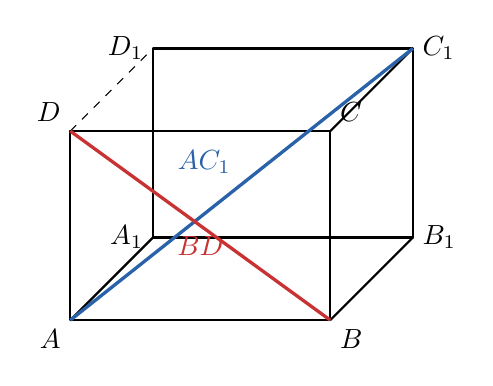
\begin{tikzpicture}[scale=1.5, line join=round]
  % 底面
  \coordinate (A) at (0,0);
  \coordinate (B) at (2.2,0);
  \coordinate (C) at (2.2,1.6);
  \coordinate (D) at (0,1.6);
  % 顶面
  \coordinate (A1) at (0.7,0.7);
  \coordinate (B1) at (2.9,0.7);
  \coordinate (C1) at (2.9,2.3);
  \coordinate (D1) at (0.7,2.3);
  % 底面
  \draw[thick] (A) -- (B) -- (C) -- (D) -- cycle;
  % 顶面
  \draw[thick] (A1) -- (B1) -- (C1) -- (D1) -- cycle;
  % 侧棱
  \draw[thick] (A) -- (A1);
  \draw[thick] (B) -- (B1);
  \draw[thick] (C) -- (C1);
  \draw[dashed] (D) -- (D1);
  % 对角线
  \draw[very thick, mainblue] (A) -- (C1) node[midway, above left] {$AC_1$};
  \draw[very thick, warnred] (B) -- (D) node[midway, below] {$BD$};
  % 标注
  \node[below left] at (A) {$A$};
  \node[below right] at (B) {$B$};
  \node[above right] at (C) {$C$};
  \node[above left] at (D) {$D$};
  \node[left] at (A1) {$A_1$};
  \node[right] at (B1) {$B_1$};
  \node[right] at (C1) {$C_1$};
  \node[left] at (D1) {$D_1$};
\end{tikzpicture}
\end{center}

% -------------------- 例题3 --------------------
\begin{examplebox}[【例题3】求平面的法向量]
已知平面 $\alpha$ 过三点 $A(1,0,0)$、$B(0,1,0)$、$C(0,0,1)$，求平面 $\alpha$ 的一个法向量。
\end{examplebox}

\textbf{解：}

在平面 $\alpha$ 内取两个不共线的向量：
\[
\overrightarrow{AB}=(-1,1,0),\quad\overrightarrow{AC}=(-1,0,1)
\]

设法向量 $\vec{n}=(x,y,z)$，则
\[
\begin{cases}\vec{n}\cdot\overrightarrow{AB}=-x+y=0\\\vec{n}\cdot\overrightarrow{AC}=-x+z=0\end{cases}
\]
解得 $y=x$，$z=x$。令 $x=1$，得 $\vec{n}=(1,1,1)$。

\begin{tipbox}[方法总结]
求平面法向量时，先在平面内找两个不共线的向量（通常用两点之间的向量），再设法向量 $\vec{n}=(x,y,z)$，利用垂直关系列方程组求解。令其中一个分量为 $1$（或其他方便的值）即可求出一个法向量。
\end{tipbox}

% -------------------- 例题4 --------------------
\begin{examplebox}[【例题4】证明线面平行]
在正方体 $ABCD$-$A_1B_1C_1D_1$ 中，$E$、$F$ 分别是 $BB_1$、$DD_1$ 的中点，棱长为 $1$。用向量方法证明 $EF\parallel$ 平面 $ABCD$。
\end{examplebox}

\textbf{解：}

以 $A$ 为原点，$\overrightarrow{AB}$、$\overrightarrow{AD}$、$\overrightarrow{AA_1}$ 方向为 $x$、$y$、$z$ 轴正方向建立空间直角坐标系。

各点坐标为：
$A(0,0,0)$，$B(1,0,0)$，$D(0,1,0)$，$A_1(0,0,1)$，$B_1(1,0,1)$，$D_1(0,1,1)$。

$E$ 为 $BB_1$ 中点：$E(1,0,\tfrac{1}{2})$；$F$ 为 $DD_1$ 中点：$F(0,1,\tfrac{1}{2})$。

\[
\overrightarrow{EF}=(-1,1,0)
\]

平面 $ABCD$ 的法向量为 $\vec{n}=\overrightarrow{AA_1}=(0,0,1)$。

由于 $\overrightarrow{EF}\cdot\vec{n}=-1\times0+1\times0+0\times1=0$，所以 $\overrightarrow{EF}\perp\vec{n}$。

又因为 $E$ 不在平面 $ABCD$ 上（$z$ 坐标为 $\tfrac{1}{2}\ne0$），所以 $EF\parallel$ 平面 $ABCD$。

% -------------------- 例题5 --------------------
\begin{examplebox}[【例题5】求二面角]
在正三棱柱 $ABC$-$A_1B_1C_1$ 中，底面边长为 $2$，侧棱长为 $2$。用向量方法求二面角 $A$-$A_1B$-$C$ 的大小。
\end{examplebox}

\textbf{解：}

以 $B$ 为原点建立空间直角坐标系。令 $\overrightarrow{BC}$ 方向为 $x$ 轴，在底面内与 $x$ 轴垂直的方向为 $y$ 轴（使得 $A$ 在 $y$ 轴正侧），$\overrightarrow{BB_1}$ 方向为 $z$ 轴。

各点坐标：
\begin{align*}
B&(0,0,0),\quad C(2,0,0),\quad A(1,\sqrt{3},0),\quad A_1(1,\sqrt{3},2)
\end{align*}

二面角 $A$-$A_1B$-$C$ 以 $A_1B$ 为棱。

$\overrightarrow{BA_1}=(1,\sqrt{3},2)$，$\overrightarrow{BA}=(1,\sqrt{3},0)$，$\overrightarrow{BC}=(2,0,0)$。

\textbf{半平面 $A_1BA$ 的法向量} $\vec{n}_1$：由 $\vec{n}_1\perp\overrightarrow{BA_1}$ 和 $\vec{n}_1\perp\overrightarrow{BA}$：
\[
\begin{cases}x+\sqrt{3}y+2z=0\\x+\sqrt{3}y=0\end{cases}\implies z=0,\;x=-\sqrt{3}y
\]
令 $y=1$，$\vec{n}_1=(-\sqrt{3},1,0)$。

\textbf{半平面 $A_1BC$ 的法向量} $\vec{n}_2$：由 $\vec{n}_2\perp\overrightarrow{BA_1}$ 和 $\vec{n}_2\perp\overrightarrow{BC}$：
\[
\begin{cases}x+\sqrt{3}y+2z=0\\2x=0\end{cases}\implies x=0,\;\sqrt{3}y+2z=0
\]
令 $y=2$，$\vec{n}_2=(0,2,-\sqrt{3})$。

\[
\cos\theta=\frac{\vec{n}_1\cdot\vec{n}_2}{|\vec{n}_1|\cdot|\vec{n}_2|}=\frac{0+2+0}{2\cdot\sqrt{4+3}}=\frac{2}{2\sqrt{7}}=\frac{1}{\sqrt{7}}=\frac{\sqrt{7}}{7}
\]

所以二面角 $A$-$A_1B$-$C$ 的大小为 $\boxed{\arccos\dfrac{\sqrt{7}}{7}}$。

\begin{center}
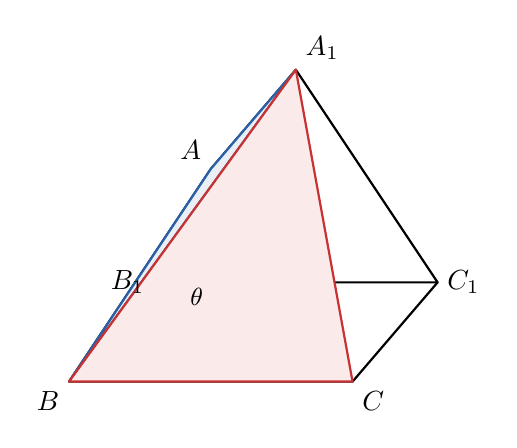
\begin{tikzpicture}[scale=1.8, line join=round]
  \coordinate (B) at (0,0);
  \coordinate (C) at (2,0);
  \coordinate (A) at (1,1.5);
  \coordinate (B1) at (0.6,0.7);
  \coordinate (C1) at (2.6,0.7);
  \coordinate (A1) at (1.6,2.2);
  \draw[thick] (A) -- (B) -- (C) -- cycle;
  \draw[thick] (A1) -- (B1) -- (C1) -- cycle;
  \draw[thick] (A) -- (A1);
  \draw[thick] (B) -- (B1);
  \draw[thick] (C) -- (C1);
  \draw[thick, mainblue, fill=mainblue!10] (A) -- (B) -- (A1) -- cycle;
  \draw[thick, warnred, fill=warnred!10] (C) -- (B) -- (A1) -- cycle;
  \node[below left] at (B) {$B$};
  \node[below right] at (C) {$C$};
  \node[above left] at (A) {$A$};
  \node[left] at (B1) {$B_1$};
  \node[right] at (C1) {$C_1$};
  \node[above right] at (A1) {$A_1$};
  \node at (0.9,0.6) {\small$\theta$};
\end{tikzpicture}
\end{center}

% -------------------- 例题6 --------------------
\begin{examplebox}[【例题6】求直线与平面所成的角]
在正方体 $ABCD$-$A_1B_1C_1D_1$ 中，棱长为 $1$。求直线 $A_1C$ 与平面 $ABCD$ 所成的角。
\end{examplebox}

\textbf{解：}

以 $A$ 为原点，$\overrightarrow{AB}$、$\overrightarrow{AD}$、$\overrightarrow{AA_1}$ 方向为 $x$、$y$、$z$ 轴正方向建立空间直角坐标系。

$A(0,0,0)$，$C(1,1,0)$，$A_1(0,0,1)$。

\[
\overrightarrow{A_1C}=(1,1,-1)
\]

平面 $ABCD$ 的法向量 $\vec{n}=(0,0,1)$。

设直线 $A_1C$ 与平面 $ABCD$ 所成的角为 $\theta$：
\[
\sin\theta=\frac{|\overrightarrow{A_1C}\cdot\vec{n}|}{|\overrightarrow{A_1C}|\cdot|\vec{n}|}=\frac{|-1|}{\sqrt{1+1+1}\cdot1}=\frac{1}{\sqrt{3}}=\frac{\sqrt{3}}{3}
\]

所以 $\theta=\arcsin\dfrac{\sqrt{3}}{3}$。

\begin{center}
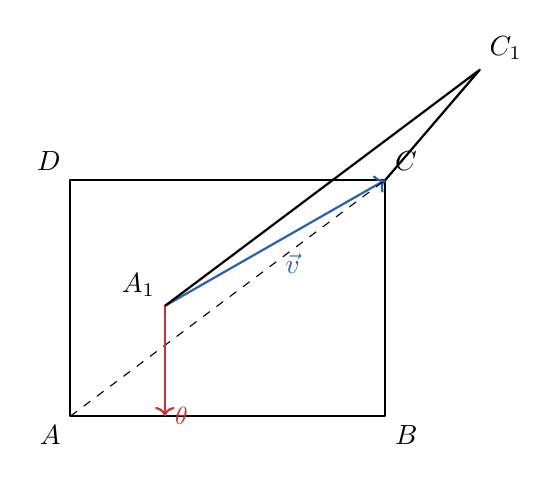
\begin{tikzpicture}[scale=2, line join=round]
  \coordinate (A) at (0,0);
  \coordinate (B) at (2,0);
  \coordinate (C) at (2,1.5);
  \coordinate (D) at (0,1.5);
  \coordinate (A1) at (0.6,0.7);
  \coordinate (C1) at (2.6,2.2);
  \draw[thick] (A) -- (B) -- (C) -- (D) -- cycle;
  \draw[thick, mainblue, ->] (A1) -- (C) node[midway, below right] {$\vec{v}$};
  \draw[dashed] (A) -- (C);
  \draw[thick, warnred, ->] (A1) -- ++(0,-0.7) node[right, font=\small] {$\theta$};
  \node[below left] at (A) {$A$};
  \node[below right] at (B) {$B$};
  \node[above right] at (C) {$C$};
  \node[above left] at (D) {$D$};
  \node[above left] at (A1) {$A_1$};
  \node[above right] at (C1) {$C_1$};
  \draw[thick] (A1) -- (C1) -- (C);
\end{tikzpicture}
\end{center}

% -------------------- 例题7 --------------------
\begin{examplebox}[【例题7】求点到平面的距离]
已知正四面体 $ABCD$ 的棱长为 $2$，求顶点 $A$ 到平面 $BCD$ 的距离。
\end{examplebox}

\textbf{解：}

以 $D$ 为原点，$\overrightarrow{DC}$ 方向为 $x$ 轴建立空间直角坐标系。正四面体棱长为 $2$，底面 $BCD$ 为正三角形。

\[
D(0,0,0),\quad C(2,0,0),\quad B(1,\sqrt{3},0)
\]

设 $A(x,y,z)$，由 $|AD|=|AB|=|AC|=2$：
\begin{align*}
x^2+y^2+z^2&=4 \quad\cdots(1)\\
(x-2)^2+y^2+z^2&=4 \quad\cdots(2)\\
(x-1)^2+(y-\sqrt{3})^2+z^2&=4 \quad\cdots(3)
\end{align*}

由 $(2)-(1)$：$-4x+4=0\implies x=1$。

代入 $(1)$：$1+y^2+z^2=4\implies y^2+z^2=3$。

代入 $(3)$：$(y-\sqrt{3})^2+z^2=4-1=3$，即 $y^2-2\sqrt{3}y+3+z^2=3$。

将 $y^2+z^2=3$ 代入：$3-2\sqrt{3}y+3=3\implies y=\dfrac{\sqrt{3}}{3}$。

$z^2=3-\dfrac{1}{3}=\dfrac{8}{3}$，$z=\dfrac{2\sqrt{6}}{3}$（取正值）。

所以 $A\!\left(1,\dfrac{\sqrt{3}}{3},\dfrac{2\sqrt{6}}{3}\right)$。

平面 $BCD$ 即 $z=0$ 平面，法向量 $\vec{n}=(0,0,1)$。

$A$ 到平面 $BCD$ 的距离：
\[
d=\frac{|\overrightarrow{DA}\cdot\vec{n}|}{|\vec{n}|}=\frac{z_A}{1}=\frac{2\sqrt{6}}{3}
\]

\begin{tipbox}[方法总结]
对于正四面体棱长为 $a$，顶点到底面的距离为 $\dfrac{a\sqrt{6}}{3}$。本题中 $a=2$，验证 $d=\dfrac{2\sqrt{6}}{3}$，结论正确。
\end{tipbox}

% -------------------- 例题8 --------------------
\begin{examplebox}[【例题8】综合题——求异面直线所成角与点到平面的距离]
在正方体 $ABCD$-$A_1B_1C_1D_1$ 中，棱长为 $2$。求：
(1) 异面直线 $A_1B$ 与 $B_1D_1$ 所成的角；
(2) 点 $A$ 到平面 $B_1CD_1$ 的距离。
\end{examplebox}

\textbf{解：}

以 $A$ 为原点，$\overrightarrow{AB}$、$\overrightarrow{AD}$、$\overrightarrow{AA_1}$ 方向为 $x$、$y$、$z$ 轴正方向建立空间直角坐标系。

各点坐标：
\begin{align*}
A&(0,0,0),\;B(2,0,0),\;C(2,2,0),\;D(0,2,0)\\
A_1&(0,0,2),\;B_1(2,0,2),\;C_1(2,2,2),\;D_1(0,2,2)
\end{align*}

\textbf{(1) 求异面直线 $A_1B$ 与 $B_1D_1$ 所成的角：}

\[
\overrightarrow{A_1B}=(2,0,-2),\quad\overrightarrow{B_1D_1}=(-2,2,0)
\]
\[
\cos\theta=\frac{|\overrightarrow{A_1B}\cdot\overrightarrow{B_1D_1}|}{|\overrightarrow{A_1B}|\cdot|\overrightarrow{B_1D_1}|}=\frac{|-4+0+0|}{\sqrt{8}\cdot\sqrt{8}}=\frac{4}{8}=\frac{1}{2}
\]

所以 $\theta=60°$。

\textbf{(2) 求点 $A$ 到平面 $B_1CD_1$ 的距离：}

$\overrightarrow{B_1C}=(0,2,-2)$，$\overrightarrow{B_1D_1}=(-2,2,0)$。

设法向量 $\vec{n}=(x,y,z)$：
\[
\begin{cases}2y-2z=0\\-2x+2y=0\end{cases}\implies y=z,\;x=y
\]
令 $x=y=z=1$，$\vec{n}=(1,1,1)$。

\[
d=\frac{|\overrightarrow{AB_1}\cdot\vec{n}|}{|\vec{n}|}=\frac{|2+0+2|}{\sqrt{3}}=\frac{4}{\sqrt{3}}=\frac{4\sqrt{3}}{3}
\]

\begin{center}
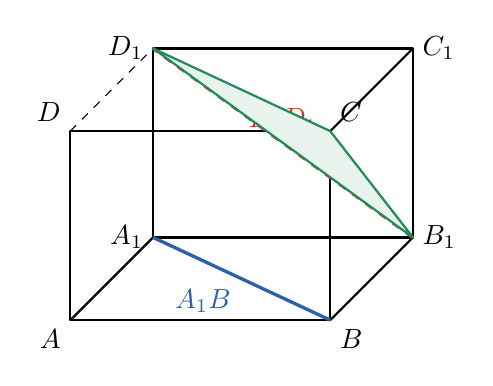
\begin{tikzpicture}[scale=1.5, line join=round]
  \coordinate (A) at (0,0);
  \coordinate (B) at (2.2,0);
  \coordinate (C) at (2.2,1.6);
  \coordinate (D) at (0,1.6);
  \coordinate (A1) at (0.7,0.7);
  \coordinate (B1) at (2.9,0.7);
  \coordinate (C1) at (2.9,2.3);
  \coordinate (D1) at (0.7,2.3);
  \draw[thick] (A) -- (B) -- (C) -- (D) -- cycle;
  \draw[thick] (A1) -- (B1) -- (C1) -- (D1) -- cycle;
  \draw[thick] (A) -- (A1) (B) -- (B1) (C) -- (C1);
  \draw[dashed] (D) -- (D1);
  \draw[very thick, mainblue] (A1) -- (B) node[midway, below left] {$A_1B$};
  \draw[very thick, warnred, dashed] (B1) -- (D1) node[midway, above] {$B_1D_1$};
  \draw[thick, tipgreen, fill=tipgreen!10] (B1) -- (C) -- (D1) -- cycle;
  \node[below left] at (A) {$A$};
  \node[below right] at (B) {$B$};
  \node[above right] at (C) {$C$};
  \node[above left] at (D) {$D$};
  \node[left] at (A1) {$A_1$};
  \node[right] at (B1) {$B_1$};
  \node[right] at (C1) {$C_1$};
  \node[left] at (D1) {$D_1$};
\end{tikzpicture}
\end{center}

% ================================================================
%  第三部分：应用题
% ================================================================
\section*{\textcolor{apppurple}{三、应用题}}

% -------------------- 应用1 --------------------
\begin{appbox}[【应用1】建筑中的角度问题]
如图，一座建筑物的屋顶可以看作一个三棱锥 $P$-$ABC$，其中底面 $ABC$ 是直角三角形，$\angle BAC=90°$，$AB=4$ 米，$AC=3$ 米，棱锥的高 $PO$（$O$ 为底面外心）垂直于底面，$PO=6$ 米。求侧面 $PAB$ 与底面 $ABC$ 所成二面角的大小。
\end{appbox}

\textbf{解：}

以 $A$ 为原点，$\overrightarrow{AB}$、$\overrightarrow{AC}$ 方向为 $x$、$y$ 轴正方向，竖直向上为 $z$ 轴正方向建立空间直角坐标系。

底面直角三角形斜边 $BC=\sqrt{16+9}=5$，外心 $O$ 为斜边 $BC$ 中点。

$A(0,0,0)$，$B(4,0,0)$，$C(0,3,0)$，$O(2,1.5,0)$，$P(2,1.5,6)$。

平面 $ABC$ 的法向量 $\vec{n}_1=(0,0,1)$。

平面 $PAB$ 内的向量：$\overrightarrow{PA}=(-2,-1.5,-6)$，$\overrightarrow{PB}=(2,-1.5,-6)$。

法向量 $\vec{n}_2=(x,y,z)$：
\[
\begin{cases}
-2x-1.5y-6z=0\\
2x-1.5y-6z=0
\end{cases}
\]
两式相减：$-4x=0\implies x=0$。代入得 $-1.5y-6z=0\implies y=-4z$。

令 $z=-1$，$y=4$，$\vec{n}_2=(0,4,-1)$。

两个法向量分别指向二面角的两侧，取正号：
\[
\cos\theta=\frac{|\vec{n}_1\cdot\vec{n}_2|}{|\vec{n}_1||\vec{n}_2|}=\frac{|0+0-1|}{\sqrt{17}}=\frac{1}{\sqrt{17}}=\frac{\sqrt{17}}{17}
\]

所以侧面 $PAB$ 与底面 $ABC$ 所成二面角的大小为 $\arccos\dfrac{\sqrt{17}}{17}$。

% -------------------- 应用2 --------------------
\begin{appbox}[【应用2】卫星太阳能板的安装角度]
某卫星的太阳能板展开后，可以近似看作一个平面。已知卫星主体为正方体，棱长为 $2$ 米。太阳能板 $S$ 过棱 $AB$ 的中点 $M$ 和棱 $A_1D_1$ 的中点 $N$，且板面垂直于底面 $ABCD$。求太阳能板 $S$ 与卫星侧面 $ABB_1A_1$ 所成的二面角。
\end{appbox}

\textbf{解：}

以 $A$ 为原点，$\overrightarrow{AB}$、$\overrightarrow{AD}$、$\overrightarrow{AA_1}$ 方向为 $x$、$y$、$z$ 轴正方向建立空间直角坐标系。

$A(0,0,0)$，$B(2,0,0)$，$D(0,2,0)$，$A_1(0,0,2)$，$D_1(0,2,2)$。

$M$ 为 $AB$ 中点：$M(1,0,0)$。$N$ 为 $A_1D_1$ 中点：$N(0,1,2)$。

$\overrightarrow{MN}=(-1,1,2)$。

太阳能板 $S$ 垂直于底面 $ABCD$，意味着 $S$ 的法向量 $\vec{n}_S$ 与底面法向量 $(0,0,1)$ 垂直，即 $\vec{n}_S=(a,b,0)$。

$\vec{n}_S\perp\overrightarrow{MN}$：$-a+b=0\implies a=b$。令 $a=b=1$，$\vec{n}_S=(1,1,0)$。

平面 $ABB_1A_1$（即 $xz$ 平面）的法向量 $\vec{n}_2=(0,1,0)$。

\[
\cos\theta=\frac{|\vec{n}_S\cdot\vec{n}_2|}{|\vec{n}_S||\vec{n}_2|}=\frac{1}{\sqrt{2}}=\frac{\sqrt{2}}{2}
\]

所以 $\theta=45°$。太阳能板 $S$ 与侧面 $ABB_1A_1$ 所成的二面角为 $45°$。

% -------------------- 应用3 --------------------
\begin{appbox}[【应用3】工业机器人臂的空间定位]
某工业机器人的机械臂可以抽象为从原点 $O$ 出发的三条线段 $OA$、$AB$、$BC$。已知 $OA$ 沿 $x$ 轴正方向，长 $3$ 米；$AB$ 在 $xy$ 平面内与 $OA$ 成 $60°$，长 $2$ 米；$BC$ 垂直于 $xy$ 平面向上，长 $1$ 米。求末端 $C$ 与基座 $O$ 之间的距离，以及 $OC$ 与底面（$xy$ 平面）所成的角。
\end{appbox}

\textbf{解：}

建立空间直角坐标系。$O(0,0,0)$。

$OA$ 沿 $x$ 轴正方向，$A(3,0,0)$。

$AB$ 在 $xy$ 平面内与 $OA$ 成 $60°$，$|AB|=2$，$B(3+2\cos60°,\;2\sin60°,\;0)=(4,\sqrt{3},0)$。

$BC$ 垂直于 $xy$ 平面向上，$|BC|=1$，$C(4,\sqrt{3},1)$。

\textbf{距离：}
\[
|OC|=\sqrt{16+3+1}=\sqrt{20}=2\sqrt{5}\approx4.47\text{ 米}
\]

\textbf{$OC$ 与底面所成的角：}

$\overrightarrow{OC}=(4,\sqrt{3},1)$，底面法向量 $\vec{n}=(0,0,1)$。

\[
\sin\alpha=\frac{|\overrightarrow{OC}\cdot\vec{n}|}{|\overrightarrow{OC}||\vec{n}|}=\frac{1}{\sqrt{20}}=\frac{1}{2\sqrt{5}}=\frac{\sqrt{5}}{10}
\]

$\alpha=\arcsin\dfrac{\sqrt{5}}{10}\approx12.9°$。

\begin{center}
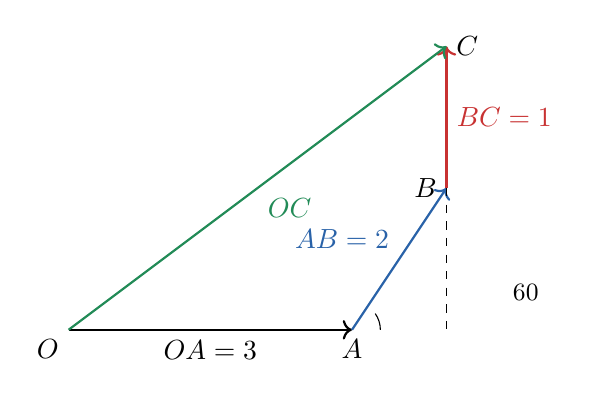
\begin{tikzpicture}[scale=1.2, line join=round]
  \draw[->, thick] (0,0) -- (3,0) node[midway, below] {$OA=3$};
  \draw[->, thick, mainblue] (3,0) -- (4,1.5) node[midway, above left] {$AB=2$};
  \draw[->, thick, warnred] (4,1.5) -- (4,3) node[midway, right] {$BC=1$};
  \draw[->, thick, tipgreen] (0,0) -- (4,3) node[midway, below right] {$OC$};
  \draw[dashed] (4,1.5) -- (4,0);
  \node at (0,0) [below left] {$O$};
  \node at (3,0) [below] {$A$};
  \node at (4,1.5) [left] {$B$};
  \node at (4,3) [right] {$C$};
  \node at (4.6,0.4) [right] {\small$60°$};
  \draw (3.3,0) arc (0:35:0.3);
\end{tikzpicture}
\end{center}

% ================================================================
%  第四部分：课堂练习
% ================================================================
\section*{\textcolor{tipgreen}{四、课堂练习}}

\begin{enumerate}
  \item 已知 $\vec{a}=(2,-1,3)$，$\vec{b}=(-1,2,1)$，求 $\vec{a}\cdot\vec{b}$、$|\vec{a}|$、$\vec{a}$ 与 $\vec{b}$ 的夹角。

  \item 在空间直角坐标系中，$A(1,2,3)$，$B(3,1,2)$，求 $|AB|$ 及 $\overrightarrow{AB}$ 的方向余弦。

  \item 已知 $\vec{a}=(1,0,-1)$，$\vec{b}=(0,1,1)$，求同时垂直于 $\vec{a}$ 和 $\vec{b}$ 的单位向量。

  \item 在正方体 $ABCD$-$A_1B_1C_1D_1$ 中，棱长为 $1$。用向量方法证明 $BD_1\perp AC$。

  \item 在正四棱锥 $S$-$ABCD$ 中，底面边长为 $2$，侧棱长为 $\sqrt{6}$。求侧面与底面所成二面角的大小。

  \item 在三棱锥 $P$-$ABC$ 中，$PA\perp$ 平面 $ABC$，$AB\perp AC$，$PA=AB=AC=1$。求点 $A$ 到平面 $PBC$ 的距离。
\end{enumerate}

\begin{knowledgebox}[参考答案]

\textbf{1.}
\[
\vec{a}\cdot\vec{b}=2\times(-1)+(-1)\times2+3\times1=-2-2+3=-1
\]
\[
|\vec{a}|=\sqrt{4+1+9}=\sqrt{14},\quad|\vec{b}|=\sqrt{1+4+1}=\sqrt{6}
\]
\[
\cos\theta=\frac{-1}{\sqrt{14}\cdot\sqrt{6}}=\frac{-1}{2\sqrt{21}}=-\frac{\sqrt{21}}{42}
\]
$\theta=\pi-\arccos\dfrac{\sqrt{21}}{42}\approx 97.6°$。

\bigskip
\textbf{2.}
\[
\overrightarrow{AB}=(2,-1,-1),\quad|AB|=\sqrt{4+1+1}=\sqrt{6}
\]
方向余弦：$\cos\alpha=\dfrac{2}{\sqrt{6}}=\dfrac{\sqrt{6}}{3}$，$\cos\beta=\dfrac{-1}{\sqrt{6}}=-\dfrac{\sqrt{6}}{6}$，$\cos\gamma=\dfrac{-1}{\sqrt{6}}=-\dfrac{\sqrt{6}}{6}$。

\bigskip
\textbf{3.}
设 $\vec{c}=(x,y,z)$ 同时垂直于 $\vec{a}$ 和 $\vec{b}$：
\[
\begin{cases}x-z=0\\y+z=0\end{cases}\implies x=z,\;y=-z
\]
令 $z=1$，$\vec{c}=(1,-1,1)$，$|\vec{c}|=\sqrt{3}$。

单位向量为 $\pm\dfrac{1}{\sqrt{3}}(1,-1,1)=\pm\!\left(\dfrac{\sqrt{3}}{3},-\dfrac{\sqrt{3}}{3},\dfrac{\sqrt{3}}{3}\right)$。

\bigskip
\textbf{4.}
以 $A$ 为原点建系。$A(0,0,0)$，$B(1,0,0)$，$C(1,1,0)$，$D(0,1,0)$，$D_1(0,1,1)$。

$\overrightarrow{BD_1}=(-1,1,1)$，$\overrightarrow{AC}=(1,1,0)$。

$\overrightarrow{BD_1}\cdot\overrightarrow{AC}=-1+1+0=0$。

所以 $BD_1\perp AC$。

\bigskip
\textbf{5.}
以底面中心 $O$ 为原点建系。底面正方形边长为 $2$，半对角线 $\sqrt{2}$。

$A(-1,-1,0)$，$B(1,-1,0)$，$C(1,1,0)$，$D(-1,1,0)$。

$S(0,0,h)$，由 $|SB|^2=1+1+h^2=6\implies h=2$，$S(0,0,2)$。

取侧面 $SBC$，$\overrightarrow{SB}=(1,-1,-2)$，$\overrightarrow{SC}=(1,1,-2)$。

法向量 $\vec{n}$：由 $\begin{cases}x-y-2z=0\\x+y-2z=0\end{cases}\implies x=2z,\;y=0$。令 $z=1$，$\vec{n}=(2,0,1)$。

底面法向量 $\vec{n}_0=(0,0,1)$。

$\cos\theta=\dfrac{|\vec{n}\cdot\vec{n}_0|}{|\vec{n}||\vec{n}_0|}=\dfrac{1}{\sqrt{5}}=\dfrac{\sqrt{5}}{5}$。

二面角为 $\arccos\dfrac{\sqrt{5}}{5}$。

\bigskip
\textbf{6.}
以 $A$ 为原点，$\overrightarrow{AB}$、$\overrightarrow{AC}$、$\overrightarrow{AP}$ 方向为 $x$、$y$、$z$ 轴正方向。

$A(0,0,0)$，$B(1,0,0)$，$C(0,1,0)$，$P(0,0,1)$。

平面 $PBC$：$\overrightarrow{PB}=(1,0,-1)$，$\overrightarrow{PC}=(0,1,-1)$。

法向量：$\begin{cases}x-z=0\\y-z=0\end{cases}\implies x=y=z$。$\vec{n}=(1,1,1)$。

$\overrightarrow{AP}=(0,0,1)$，$d=\dfrac{|\overrightarrow{AP}\cdot\vec{n}|}{|\vec{n}|}=\dfrac{1}{\sqrt{3}}=\dfrac{\sqrt{3}}{3}$。

\end{knowledgebox}

\vfill
\begin{center}
\small\textcolor{gray}{本讲义仅供教学参考，例题可根据学生水平调整难度。}
\end{center}

\end{document}
